% =====================================================================
%  IEEE Transactions on Computational Social Systems -- resubmission
%  Built on the official IEEE template (bare_jrnl_new_sample4.tex,
%  IEEEtran.cls V1.8b). Compile with pdfLaTeX + BibTeX (IEEEtran.bst).
%  All numbers in tables come from make_tables.py (results CSVs).
%  Red [ ... ] marks the remaining placeholders (code URL, AI-use
%  disclosure). Before submission: \renewcommand{\res}[1]{#1} and
%  check that no red text remains.
% =====================================================================
\documentclass[lettersize,journal]{IEEEtran}
\usepackage{amsmath,amsfonts,amssymb}
\usepackage{array}
\usepackage{textcomp}
\usepackage{stfloats}
\usepackage{url}
\usepackage{verbatim}
\usepackage{graphicx}
\usepackage{cite}
\usepackage{booktabs}
\usepackage{multirow}
\usepackage[table]{xcolor}
% clickable citations, table/figure/section references and URLs
% (hidelinks keeps the IEEE look: no coloured boxes)
\usepackage[hidelinks]{hyperref}
\hyphenation{op-tical net-works semi-conduc-tor IEEE-Xplore}

\newcommand{\res}[1]{\textcolor{red}{[#1]}}
\newcommand{\tbd}{\res{--}}

\begin{document}

\title{Who Handles the Uncertain Cases? Confidence-Based Human--AI Triage for Hate Speech Moderation}

\author{Kolla~Jeevan,
        V.~S.~Abhinay~Paul,
        and~Angotu~Nageswara~Rao,~\IEEEmembership{Member,~IEEE}%
\thanks{Manuscript received xxxx xx, 2026; revised xxxx xx, 2026.}%
\thanks{K.~Jeevan, V.~S.~A.~Paul, and A.~N.~Rao are with the Department of Computer Science and Engineering (AI\&ML), Geethanjali College of Engineering and Technology, Cheeriyal~(V), Keesara~(M), Medchal~Malkajgiri~(D), Hyderabad, Telangana, India~--~501301 (e-mail: 20r11a6627@gcet.edu.in; 20r11a6658@gcet.edu.in; dranrao.cse@gcet.edu.in).}%
\thanks{Corresponding author: A.~N.~Rao (ORCID: 0000-0002-8413-5994). K.~Jeevan (ORCID: \res{Jeevan's ORCID}). V.~S.~A.~Paul (ORCID: 0009-0004-6726-2272).}}

\markboth{IEEE Transactions on Computational Social Systems}%
{Jeevan \MakeLowercase{\textit{et al.}}: Confidence-Based Human--AI Triage for Hate Speech Moderation}

\maketitle

\begin{abstract}
Platforms moderate hate speech through a division of labor: classifiers decide the posts they are confident about, and human moderators review the rest. Yet detectors are almost always evaluated as stand-alone classifiers. We evaluate the moderation pipeline as a whole on two benchmarks (Davidson, 24,783 tweets; HateXplain, 19,229 posts), comparing classical, bio-inspired multi-stage, and transformer classifiers over five leakage-free splits and simulating deferral of the least-confident posts to human moderators whose decisions are drawn from the datasets' real annotator votes. Transformers exceed the best classical models by 0.054--0.062 macro-F1, while a zero-shot 3B-parameter LLM trails every fine-tuned model (0.39--0.51) because it labels much non-hate as hate. Macro-F1 also hides missed hate: on Davidson, unweighted transformers miss 57\% of hate posts, whereas class-weighted logistic regression misses 40\% and class-weighted HateBERT 46\% at unchanged macro-F1. Reviewing the 10\% least-confident posts lets a CPU-only class-weighted SVM match a transformer working alone, and a cascade sends only 19--42\% of posts to a GPU; missed hate falls only modestly, because most missed hate is predicted with high confidence. Confidence-based deferral sends tweets in White-aligned English to review 1.7--3.3 times as often as tweets in African-American English, so review widens the dialect gap in false abusive flags (from 5.8 to 8.2 times for BERTweet), in 11 of 12 model--threshold settings. A reproducibility audit of a published multi-stage pipeline finds that its swarm feature selection, genetic tuning, and fuzzy post-processor add nothing over class weighting, and that computing feature-selection fitness on the test split inflates macro-F1 by 0.010--0.012.
\end{abstract}

\begin{IEEEkeywords}
Content moderation, hate speech, human--AI collaboration, learning to defer, algorithmic fairness, dialect bias, fuzzy logic, transformers.
\end{IEEEkeywords}

% =====================================================================
\section{Introduction}
% =====================================================================
\IEEEPARstart{H}{ate} speech moderation at platform scale is a socio-technical system rather than a classifier. Automated filters screen millions of posts, but the decisions that are hardest, and often the most consequential for the people targeted, are routed to human moderators \cite{gillespie2018custodians,gorwa2020algorithmic}. This arrangement has three costs that no single accuracy number captures. Hate that the system does not catch remains visible to its targets. Every post routed to a person adds to a workload that is known to harm moderators' psychological well-being \cite{roberts2019behind,steiger2021psychological}. And the errors of automated classifiers are not evenly distributed: tweets written in African-American English (AAE) are substantially more likely to be labeled offensive or hateful, both by annotators and by models trained on their labels \cite{sap2019risk,davidson2019racial}.

The hate speech detection literature has nevertheless focused on improving the stand-alone classifier. A representative example is the multi-stage pipeline of Ketsbaia \textit{et al.} \cite{ketsbaia2023multistage}, which combines TF-IDF classifiers with particle swarm feature selection, genetic hyper-parameter search, and a fuzzy post-processor for low-confidence predictions. That design already contains the core idea of moderation triage, since some predictions are trusted and others are routed elsewhere, but it routes uncertain posts to another algorithm rather than to a person and is evaluated only by aggregate macro-F1.

This paper treats the routing decision as the object of study. We ask four questions.

\textbf{RQ1.} Under a leakage-free, multi-split protocol with calibrated confidence, how do classical models, the bio-inspired multi-stage pipeline, fine-tuned transformers, and a zero-shot large language model (LLM) compare, overall and on the hate class?

\textbf{RQ2.} For a given human review budget, how much hate does a human--AI system miss, at what expected cost, and with how much GPU computation, for single-model and cascaded designs?

\textbf{RQ3.} How are automated errors and the human review burden distributed across dialect groups and across the communities that hate speech targets?

\textbf{RQ4.} Do the components of the multi-stage pipeline add value, and how much does computing feature-selection fitness on the test split inflate reported performance?

Our main findings are as follows.
\begin{enumerate}
\item Macro-F1 and missed hate rank systems differently. Class weighting barely changes the macro-F1 of HateBERT but lowers its missed-hate rate on Davidson from 0.573 to 0.462, and a class-weighted logistic regression misses less hate (0.403) than any unweighted transformer (Section~\ref{sec:rq1}).
\item Human review substitutes for model capacity in aggregate accuracy: a CPU-only class-weighted SVM with 10\% review matches BERTweet working alone. But deferring the least-confident posts reduces missed hate slowly, even with an error-free reviewer, because most missed hate is confidently mislabeled as offensive (Section~\ref{sec:rq2}).
\item Confidence-based deferral is not neutral across dialects. It routes White-aligned English (WAE) tweets to human review more often than AAE tweets, so human review corrects WAE errors disproportionately and widens the AAE/WAE gap in false abusive flags (Section~\ref{sec:rq3}).
\item In the multi-stage pipeline, genetic tuning rediscovers class-weighted logistic regression, swarm feature selection learns which features matter but cannot change how many it keeps, and the sentiment-driven fuzzy post-processor increases missed hate. Test-set fitness inflates macro-F1 by about 0.01, more than the gap between the two best classical models (Sections~\ref{sec:leak} and \ref{sec:fuzzyres}).
\end{enumerate}
Methodologically, we contribute a formalization of moderation as budgeted, confidence-based deferral with a human moderator simulated from real item-level annotator votes; a redesigned three-class Mamdani fuzzy resolver; and an evaluation over two datasets, five splits, and corrected significance tests. All code is released.

\section{Related Work}
% =====================================================================
\subsection{Content Moderation as a Socio-Technical System}
Research on platform governance describes moderation as a layered process in which automated tools, platform staff, outsourced contractors, and volunteer moderators share decisions \cite{gillespie2018custodians,gorwa2020algorithmic}. Jhaver \textit{et al.} \cite{jhaver2019human} show how Reddit moderators configure and supervise automated rules, and Lai \textit{et al.} \cite{lai2022human} study conditional delegation, in which humans specify which cases a model may decide alone. The human side of this division of labor carries measurable costs: repeated exposure to abusive content is associated with psychological harm to moderators \cite{roberts2019behind,steiger2021psychological}. Our work quantifies the trade-off between these human costs and the harm of missed hate for concrete model choices.

\subsection{Selective Classification and Learning to Defer}
Abstaining on uncertain inputs dates to Chow's error--reject trade-off \cite{chow1970optimum}. Selective classification controls risk at a target coverage \cite{geifman2017selective}, and learning-to-defer methods train a model jointly with a policy for handing cases to an expert \cite{madras2018predict,mozannar2020consistent}. Madras \textit{et al.} \cite{madras2018predict} note that deferral can change the fairness of a system, not only its accuracy. Deferral policies are only as good as the model's confidence estimates, which motivates calibration \cite{guo2017calibration}. We adopt the simplest deployable policy, deferral of the least-confident posts under a fixed budget, and evaluate it with an imperfect human drawn from real annotations.

\subsection{Hate Speech Detection}
Early work combined lexical features with linear classifiers \cite{davidson2017automated,fortuna2018survey}. Bio-inspired optimizers have been used for feature selection in this setting \cite{baydogan2021metaheuristic}, and fuzzy inference has been used to resolve ambiguous instances, including in this journal \cite{liu2019fuzzy}. Ketsbaia \textit{et al.} \cite{ketsbaia2023multistage} combine both in a multi-stage pipeline, which we re-implement and extend. Transformers now dominate the task. HateBERT continues BERT pre-training on abusive Reddit communities \cite{caselli2021hatebert}, BERTweet is pre-trained on English tweets \cite{nguyen2020bertweet}, and RoBERTa is a strong general-domain baseline \cite{liu2019roberta}. Instruction-tuned LLMs can classify hate speech zero-shot with sensitivity to prompt design \cite{plazadelarco2023respectful}. Functional tests reveal systematic weaknesses that aggregate metrics hide \cite{rottger2021hatecheck}.

\subsection{Bias in Hate Speech Detection}
Sap \textit{et al.} \cite{sap2019risk} and Davidson \textit{et al.} \cite{davidson2019racial} show, using the dialect model of Blodgett \textit{et al.} \cite{blodgett2016demographic}, that AAE tweets are disproportionately labeled and predicted as abusive in several benchmarks, including the Davidson corpus used here. Dixon \textit{et al.} \cite{dixon2018measuring} define unintended bias through error-rate differences across identity terms. Prior bias analyses examine classifiers alone; we examine whether a human review stage reduces or redistributes these disparities.

\subsection{Leakage and Reproducibility}
Leakage between training and evaluation data is a widespread cause of irreproducible machine learning results \cite{kapoor2023leakage}, and NLP results often vary across random seeds by more than the differences reported between methods \cite{dodge2019show}. Wrapper-based feature selection is particularly exposed because its fitness function requires labeled evaluation data. We use multiple splits, report variance, and quantify the effect of leakage directly.

% =====================================================================
\section{Problem Formulation}\label{sec:formulation}
% =====================================================================
Let $x$ be a post with gold label $y \in \{\textsc{h},\textsc{o},\textsc{n}\}$ (hate, offensive, neither), and let a classifier output calibrated class probabilities $\tilde{\mathbf{p}}(x)$. The confidence-based uncertainty of a post is
\begin{equation}
u(x) = 1 - \max_k \tilde{p}_k(x).
\end{equation}

\textbf{Budgeted deferral.} A platform can afford to review a fraction $b$ of incoming posts. Given $N$ posts, the deferral set $\mathcal{D}_b$ contains the $\lceil bN \rceil$ posts with the largest $u(x)$. The system decision is
\begin{equation}
\hat{y}(x) =
\begin{cases}
h(x) & x \in \mathcal{D}_b,\\
\arg\max_k \tilde{p}_k(x) & \text{otherwise.}
\end{cases}
\end{equation}

\textbf{Simulated moderator.} Both datasets record how many annotators chose each label for each post. Let $\mathbf{v}(x)$ be this vote vector. We model a single human moderator as one randomly chosen annotator:
\begin{equation}
h(x) \sim \mathrm{Categorical}\!\left(\mathbf{v}(x)/\lVert \mathbf{v}(x)\rVert_1\right).
\end{equation}
The simulated human therefore errs more on posts that annotators disagreed about, which is a more realistic assumption than a perfect oracle. All triage metrics are averaged over 20 draws. We also report the oracle case $h(x)=y$ as an upper bound.

\textbf{Outcome measures.} For a budget $b$ we report the review workload $W(b)=|\mathcal{D}_b|/N$, the missed-hate rate $\mathrm{MHR}=\Pr(\hat{y}\neq\textsc{h}\mid y=\textsc{h})$, the false hate-flag rate $\mathrm{FFR}=\Pr(\hat{y}=\textsc{h}\mid y\neq\textsc{h})$, macro-F1, and an expected cost per post
\begin{equation}
J(b) = \frac{1}{N}\sum_{i=1}^{N} c\bigl(y_i,\hat{y}_i\bigr) + \lambda_r W(b),
\end{equation}
where $c(\textsc{h},\cdot)=c_m$ for missed hate, $c(\cdot,\textsc{h})=c_f=1$ for a false hate flag, $c=0.5$ for offensive/neither confusion, $c(y,y)=0$, and $\lambda_r=0.2$ is the cost of one human review relative to a false flag. Because the relative harm of missed hate is a policy choice, we sweep $c_m \in \{1,2,5,10,20\}$ and report the cost-minimizing budget for each.

\textbf{Cascade.} A cascade first applies a cheap TF-IDF model and escalates a post to a transformer only if $\max_k \tilde{p}^{\,\mathrm{cheap}}_k(x)<\tau$. The threshold $\tau$ is the value with the smallest escalation share whose validation macro-F1 is within $0.005$ of applying the transformer to every post. Human deferral is then applied to the final-stage probabilities. We report the share of posts that require GPU inference.

% =====================================================================
% =====================================================================
\section{Data}
% =====================================================================
\subsection{Datasets}
\textbf{Davidson} \cite{davidson2017automated} contains 24,783 English tweets sampled with a hate speech lexicon and labeled by at least three crowd workers as hate speech, offensive language, or neither. We use the complete released corpus. \textbf{HateXplain} \cite{mathew2021hatexplain} contains posts from Twitter and Gab labeled by three annotators as hate, offensive, or normal, together with the communities each post targets. Following its authors, we drop posts without a majority label, leaving 19,229. A target group is assigned to a post when at least two annotators named it. Table~\ref{tab:data} summarizes both corpora. They differ in two ways that matter for moderation: hate is rare in Davidson (5.8\%) but common in HateXplain (30.9\%), and annotators agree unanimously on 70.5\% of Davidson tweets but only 51.2\% of HateXplain posts.

\begin{table}[t]
\centering
\caption{Dataset Statistics}
\label{tab:data}
\footnotesize
\setlength{\tabcolsep}{3pt}
\begin{tabular}{lrr}
\toprule
 & Davidson & HateXplain \\
\midrule
Posts & 24,783 & 19,229 \\
Hate & 1,430 (5.8\%) & 5,935 (30.9\%) \\
Offensive & 19,190 (77.4\%) & 5,480 (28.5\%) \\
Neither / normal & 4,163 (16.8\%) & 7,814 (40.6\%) \\
Exact duplicate texts & 0 & 37 \\
Unanimous annotator label & 70.5\% & 51.2\% \\
Train / val.\ / test per split & 17,347/2,479/4,957 & 13,460/1,923/3,846 \\
\bottomrule
\end{tabular}

\end{table}

\subsection{Splits and Leakage Control}
Each dataset is split five times (seeds 42, 123, 456, 789, 1011) into stratified training (70\%), validation (10\%), and test (20\%) partitions. The validation partition is the only data used for feature-selection fitness, temperature scaling, the cascade threshold, and the fuzzy routing threshold. The genetic search uses cross-validation within the training partition. Each test partition is used once, for final evaluation.

\subsection{Dialect Estimation}
To study dialect disparities on Davidson, we apply the demographic dialect model of Blodgett \textit{et al.} \cite{blodgett2016demographic}, which estimates for each tweet the proportions of AAE, Hispanic, Other, and WAE language. It covers 24,685 of the 24,783 tweets (99.6\%); the rest contain no in-vocabulary word. As in prior dialect analyses of this corpus \cite{sap2019risk,davidson2019racial}, we use these posteriors to form groups. A tweet is assigned to the AAE or WAE group when the corresponding posterior is at least $0.5$, that is, when at least half of its estimated language is of that variety. This yields 8,099 AAE and 3,534 WAE tweets. At a stricter threshold of $0.8$ only 39 tweets qualify as WAE, too few for analysis, so we report thresholds $0.6$ (5,053 / 1,625) and $0.7$ (2,484 / 512) as robustness checks. Dialect estimates describe language, not the race or identity of authors, and are used only in aggregate.

\section{Models}
% =====================================================================
\subsection{TF-IDF Features}
Text for the classical models is lowercased, URLs, user mentions, retweet markers and HTML entities are removed, hashtag symbols are dropped while their words are kept, and non-alphabetic characters are removed. We use the scikit-learn \cite{pedregosa2011scikit} TF-IDF implementation fitted on the training partition with unigrams and bigrams, English stop words removed, a minimum document frequency of 2, and the 5,000 most frequent terms. For term $t$ in document $d$, with $N_d$ training documents and document frequency $\mathrm{df}(t)$,
\begin{equation}
w_{t,d} = \mathrm{tf}(t,d)\left(\ln\frac{1+N_d}{1+\mathrm{df}(t)}+1\right),
\end{equation}
where $\mathrm{tf}$ is the raw count, and each document vector is $\ell_2$-normalized.

\subsection{Classical Classifiers}
\textbf{Multinomial naive Bayes (MNB)} with Laplace smoothing ($\alpha=1$). \textbf{Logistic regression (LR)} uses the multinomial (softmax) formulation
\begin{equation}
P(y=k\mid\mathbf{x}) = \frac{\exp(\mathbf{w}_k^{\top}\mathbf{x}+b_k)}{\sum_{j}\exp(\mathbf{w}_j^{\top}\mathbf{x}+b_j)},
\end{equation}
trained by minimizing $-\sum_i \omega_{y_i}\log P(y_i\mid\mathbf{x}_i) + \frac{1}{2C}\lVert\mathbf{W}\rVert_2^2$ with $C=1$. \textbf{Linear SVM} uses $C=1$; its class scores are the softmax of the one-vs-rest decision values, so the predicted class is the SVM's own decision, and the scores are then calibrated like those of every other model. For the \textit{class-weighted} variants (suffix ``-bal''), $\omega_c = N/(K N_c)$ for $K=3$ classes with $N_c$ training examples in class $c$; otherwise $\omega_c=1$. The MNB analogue is a uniform class prior.

\subsection{Binary Particle Swarm Feature Selection}
Each particle $\mathbf{x}_s \in \{0,1\}^{D}$, $D=5{,}000$, encodes a feature subset \cite{kennedy1997discrete}. Velocities are updated as
\begin{equation}
\mathbf{v}_s \leftarrow w(t)\,\mathbf{v}_s + c_1\mathbf{r}_1\odot(\mathbf{p}_s-\mathbf{x}_s) + c_2\mathbf{r}_2\odot(\mathbf{l}_s-\mathbf{x}_s),
\end{equation}
clamped to $[-v_{\max},v_{\max}]$ with $v_{\max}=4$, where $\mathbf{p}_s$ is the particle's best position, $\mathbf{l}_s$ the best position in a ring neighborhood of five particles, $\mathbf{r}_1,\mathbf{r}_2 \sim U(0,1)^D$, and $c_1=c_2=2$. The inertia decreases linearly from $0.9$ to $0.4$ \cite{shi1998modified}:
\begin{equation}
w(t) = w_{\mathrm{s}} - (w_{\mathrm{s}}-w_{\mathrm{e}})\frac{t}{T-1}.
\end{equation}
Bits are sampled as $x_{s,j}=1$ with probability $\sigma(v_{s,j})=1/(1+e^{-v_{s,j}})$. The fitness to be minimized is
\begin{equation}
f(\mathbf{x}) = \alpha\bigl(1-F_1^{\mathrm{val}}(\mathbf{x})\bigr) + (1-\alpha)\frac{\lVert\mathbf{x}\rVert_1}{D},\quad \alpha=0.88,
\end{equation}
where $F_1^{\mathrm{val}}$ is the validation macro-F1 of the base classifier trained on the selected features. We use 20 particles and 30 iterations, with LR-bal and MNB as base classifiers. As a control, we train the same base classifier on a \textit{random} feature subset of exactly the size BPSO selected on the same split; if BPSO did not outperform this control, the swarm would not have learned which features to keep.

\subsection{Genetic Hyper-Parameter Search}
We search the space of the original pipeline \cite{ketsbaia2023multistage} (MNB with $\alpha\in[10^{-3},10^{2}]$; LR with $C\in[10^{-4},25]$), extended with the class-weighting switch. A genome is (model family, $\log_{10}$ hyper-parameter, class-weight flag). Fitness is five-fold cross-validated macro-F1 on the training partition. We use a population of 20 for 10 generations, tournament selection (size 3), two elites, blend crossover of the log-parameter, Gaussian mutation ($\sigma=0.5$, probability 0.3), and a class-weight flip with probability 0.1. After the tenth generation the bred population is evaluated once more and its best genome is retained. We implement this search directly rather than with TPOT so that every operator is specified.

\subsection{Three-Class Mamdani Fuzzy Resolver}\label{sec:fuzzydesign}
The fuzzy stage of \cite{ketsbaia2023multistage} resolves low-confidence predictions using sentiment. In our earlier implementation its output covered only hate and non-hate, so every low-confidence offensive post was necessarily misclassified. We redesign it with three consequents. The inputs are the classifier's $\tilde{p}_{\textsc{h}}$ and $\tilde{p}_{\textsc{n}}$ and the VADER negativity score \cite{hutto2014vader}. Inputs use triangular membership functions
\begin{equation}
\mu(z;a,b,c) = \max\!\left(0,\min\!\left(\tfrac{z-a}{b-a},\tfrac{c-z}{c-b}\right)\right).
\end{equation}
For the two probabilities, Low $=(0,0,0.4)$, Medium $=(0.2,0.5,0.8)$, and High $=(0.6,1,1)$. Because VADER negativity is concentrated near zero, its breakpoints are set from the 33rd, 66th, and 90th percentiles $(q_{33},q_{66},q_{90})$ of nonzero training scores: Low $=(0,0,q_{66})$, Medium $=(q_{33}/2,q_{66},q_{90})$, and High $=(q_{66},q_{90},1)$. Table~\ref{tab:rules} lists the nine rules. Inference uses minimum for conjunction and implication and maximum for aggregation \cite{mamdani1975experiment}. The output severity $s\in[0,10]$ has consequents Neither $(0,0,4)$, Offensive $(3,5,7)$, and Hate $(6,10,10)$. Defuzzification uses the centroid, and $s<3.5$, $3.5\le s<6.5$, and $s\ge6.5$ map to neither, offensive, and hate. Posts with $\max_k\tilde{p}_k<\theta$ are resolved by this stage. We report both the original $\theta=0.6$ and $\theta$ selected on validation.

\begin{table}[t]
\centering
\caption{Mamdani Rule Base of the Three-Class Fuzzy Resolver}
\label{tab:rules}
\begin{tabular}{clllc}
\toprule
Rule & $\tilde{p}_{\textsc{h}}$ & $\tilde{p}_{\textsc{n}}$ & VADER neg. & Output \\
\midrule
R1 & High & -- & -- & Hate \\
R2 & Medium & -- & High & Hate \\
R3 & Medium & -- & Medium & Offensive \\
R4 & Medium & -- & Low & Offensive \\
R5 & Medium & High & -- & Neither \\
R6 & Low & High & -- & Neither \\
R7 & Low & Medium & Low & Neither \\
R8 & Low & Medium & Medium or High & Offensive \\
R9 & Low & Low & -- & Offensive \\
\bottomrule
\end{tabular}
\end{table}

\subsection{Transformers and Zero-Shot LLM}
We fine-tune HateBERT (\texttt{GroNLP/hateBERT}) \cite{caselli2021hatebert}, RoBERTa-base \cite{liu2019roberta}, and BERTweet-base \cite{nguyen2020bertweet} with the Hugging Face Transformers library \cite{wolf2020transformers}: three epochs, learning rate $2\times10^{-5}$, batch size 16, weight decay 0.01, 6\% linear warm-up, maximum length 128, mixed precision (fp16), and the checkpoint with best validation macro-F1. HateBERT is also trained with class-weighted cross-entropy (HateBERT-w). For transformer inputs, URLs and user mentions are replaced by placeholder tokens and casing and punctuation are kept.

As a zero-shot baseline we prompt Qwen2.5-3B-Instruct \cite{qwen2024qwen25} in 16-bit precision with definitions of the three categories adapted from \cite{davidson2017automated} and ask for a single option letter. Instead of parsing generated text, we take the next-token probabilities of the three letters, renormalized, as class probabilities, which makes the model usable for calibration and deferral like every other model. Because the prompt does not depend on the split, each post is scored once and the scores are reused across splits. A 7B model was not used because, on the 16\,GB GPU available to us, it fits only in 4-bit quantization, which was too slow to score both corpora. The full prompt is given in the supplementary material.

\subsection{Calibration}
Deferral depends on confidence, so every model's probabilities are temperature-scaled \cite{guo2017calibration}: we fit a single temperature $T$ on the validation partition by minimizing negative log-likelihood of $\mathrm{softmax}(\log\mathbf{p}/T)$. Temperature scaling does not change the predicted class. We report expected calibration error (ECE, 15 bins) before and after scaling.

% =====================================================================
% =====================================================================
\section{Experimental Setup}
% =====================================================================
All experiments ran on Google Colaboratory. Classical models, swarm and genetic search, fuzzy inference, and all analyses used a CPU runtime with two virtual cores; transformers and the LLM used a single NVIDIA T4 GPU (16\,GB). Software, as provided by Colab at the time: Python 3.13, scikit-learn 1.6.1, PyTorch 2.11.0, Transformers 5.18.0 for fine-tuning and 5.22.0 for LLM scoring (the environment was updated between sessions), and vaderSentiment 3.3.2. All metrics use \texttt{zero\_division=0}, so a class that is never predicted receives precision 0. We report the missed-hate rate (MHR, $1-$hate recall) alongside macro-F1 throughout.

\textbf{Statistical testing.} Results are mean $\pm$ standard deviation over the five splits. Because random splits overlap, we compare models with the corrected resampled $t$-test \cite{nadeau2003inference}. When a family of models is compared with one reference, $p$-values are Holm-adjusted. We also computed exact McNemar tests \cite{dietterich1998approximate} within each split; because McNemar compares per-post correctness, it tracks accuracy rather than macro-F1 and can disagree with the $t$-test on macro-F1 when models trade majority-class accuracy for minority-class recall. We therefore use the $t$-test for all claims about macro-F1 and hate recall.

% =====================================================================
\section{Results}
% =====================================================================
\subsection{RQ1: Classifier Comparison}\label{sec:rq1}
Table~\ref{tab:main} reports test performance.

\begin{table*}[t]
\centering
\caption{Test Performance, Mean $\pm$ Standard Deviation of Macro-F1 Over Five Stratified Splits (Other Columns Are Means). MHR = Missed-Hate Rate ($1-$Hate Recall) With No Human Review. ECE After Temperature Scaling. Bold: Best Macro-F1 and Lowest MHR per Dataset Among Fine-Tuned Models (the LLM's Low MHR Comes From Flagging a Large Share of All Posts as Hate). $^{\dagger}$: Not Significantly Different From HateBERT (Holm-Adjusted Corrected $t$-Test, $p\ge0.05$); All Unmarked Models Are Significantly Worse.}
\label{tab:main}
\small
\setlength{\tabcolsep}{4pt}
\begin{tabular}{l|cccc|cccc}
\toprule
 & \multicolumn{4}{c|}{Davidson} & \multicolumn{4}{c}{HateXplain} \\
Model & Macro-F1 & F1 hate & MHR & ECE & Macro-F1 & F1 hate & MHR & ECE \\
\midrule
\multicolumn{9}{l}{\textit{Classical}} \\
MNB & 0.519\,$\pm$\,0.006 & 0.017 & 0.992 & 0.027 & 0.590\,$\pm$\,0.007 & 0.688 & 0.319 & 0.020 \\
MNB-bal & 0.691\,$\pm$\,0.007 & 0.357 & 0.521 & 0.030 & 0.607\,$\pm$\,0.006 & 0.691 & 0.279 & 0.021 \\
LR & 0.686\,$\pm$\,0.012 & 0.270 & 0.823 & 0.016 & 0.628\,$\pm$\,0.011 & 0.725 & 0.288 & 0.024 \\
LR-bal & 0.720\,$\pm$\,0.008 & 0.399 & \textbf{0.403} & 0.028 & 0.636\,$\pm$\,0.011 & 0.724 & 0.278 & 0.027 \\
Linear SVM & 0.708\,$\pm$\,0.014 & 0.337 & 0.743 & 0.017 & 0.609\,$\pm$\,0.008 & 0.700 & 0.301 & 0.020 \\
Linear SVM-bal & 0.726\,$\pm$\,0.009 & 0.395 & 0.578 & 0.018 & 0.610\,$\pm$\,0.009 & 0.697 & 0.299 & 0.022 \\
\midrule
\multicolumn{9}{l}{\textit{Bio-inspired}} \\
GA-selected & 0.720\,$\pm$\,0.008 & 0.399 & 0.413 & 0.026 & 0.643\,$\pm$\,0.006 & 0.729 & 0.273 & 0.034 \\
BPSO + MNB & 0.454\,$\pm$\,0.004 & 0.007 & 0.997 & 0.058 & 0.554\,$\pm$\,0.007 & 0.656 & 0.391 & 0.021 \\
BPSO + LR-bal & 0.682\,$\pm$\,0.010 & 0.361 & 0.432 & 0.039 & 0.612\,$\pm$\,0.009 & 0.695 & 0.331 & 0.023 \\
\midrule
\multicolumn{9}{l}{\textit{Transformer}} \\
RoBERTa & 0.761\,$\pm$\,0.010$^{\dagger}$ & 0.437 & 0.603 & 0.018 & 0.691\,$\pm$\,0.006$^{\dagger}$ & 0.776 & \textbf{0.192} & 0.032 \\
BERTweet & \textbf{0.780\,$\pm$\,0.007}$^{\dagger}$ & 0.475 & 0.574 & 0.016 & \textbf{0.705\,$\pm$\,0.005}$^{\dagger}$ & 0.783 & 0.212 & 0.042 \\
HateBERT & 0.772\,$\pm$\,0.009$^{\dagger}$ & 0.470 & 0.573 & 0.017 & 0.696\,$\pm$\,0.009$^{\dagger}$ & 0.782 & 0.200 & 0.035 \\
HateBERT-w & 0.774\,$\pm$\,0.006$^{\dagger}$ & 0.489 & 0.462 & 0.028 & 0.696\,$\pm$\,0.008$^{\dagger}$ & 0.783 & 0.192 & 0.038 \\
\midrule
\multicolumn{9}{l}{\textit{LLM}} \\
Qwen2.5-3B (zero-shot) & 0.510\,$\pm$\,0.005 & 0.209 & 0.147 & 0.057 & 0.393\,$\pm$\,0.004 & 0.583 & 0.117 & 0.032 \\
\bottomrule
\end{tabular}

\end{table*}

\textbf{Transformers versus classical models.} The four fine-tuned transformers are statistically indistinguishable from one another on both datasets. BERTweet has the highest mean (0.780 and 0.705), but its margin over HateBERT is not significant ($p=0.29$ and $0.15$). Pre-training on abusive Reddit communities therefore gives HateBERT no measurable advantage over general-domain RoBERTa or Twitter-domain BERTweet here. Every classical and bio-inspired model is significantly worse than HateBERT on both datasets. The gap between the best transformer and the best classical model is 0.054 on Davidson (BERTweet vs.\ SVM-bal, $p=0.002$) and 0.062 on HateXplain (BERTweet vs.\ GA-selected, $p<0.001$).

\textbf{Class weighting.} Inverse-frequency class weights help in proportion to class imbalance. On Davidson, where hate is 5.8\% of posts, weighting raises LR macro-F1 by 0.033 ($p=0.010$) and MNB by 0.173 ($p<0.001$), and raises hate recall of LR from 0.177 to 0.597 ($p<0.001$) and of SVM from 0.257 to 0.422 ($p<0.001$; its macro-F1 gain of 0.019 is not significant, $p=0.057$). On the more balanced HateXplain, the gains are 0.007 for LR ($p=0.013$), 0.017 for MNB ($p<0.001$), and none for SVM ($p=0.51$); there, weighting mainly improves the offensive class, which is HateXplain's smallest.

\textbf{Macro-F1 hides missed hate.} The model with the best macro-F1 is not the one that misses the least hate. On Davidson, unweighted transformers miss 57--60\% of hate posts, whereas LR-bal misses 40\%. Class weighting leaves HateBERT's macro-F1 unchanged ($+0.002$, $p=0.73$) but raises its hate recall by 0.111 ($p=0.010$), cutting its MHR from 0.573 to 0.462; the remaining difference between HateBERT-w and LR-bal in hate recall is not significant ($p=0.083$). On HateXplain, where hate is common, all transformers already reach MHR of about 0.19--0.21 and weighting changes little.

\textbf{Calibration.} Temperature scaling on the validation split reduces ECE substantially for poorly calibrated models (e.g., Linear SVM on Davidson from 0.103 to 0.017, MNB-bal from 0.175 to 0.030). After scaling, every model in Table~\ref{tab:main} has ECE of at most 0.058, so confidence-based deferral compares like with like.

\textbf{Zero-shot LLM.} Prompted Qwen2.5-3B reaches macro-F1 of only 0.510 on Davidson and 0.393 on HateXplain, far below every fine-tuned model ($p<0.001$ against HateBERT on both). Its errors are one-sided: it assigns the hate label to a large share of posts, with hate recall of 0.853 and 0.883 but hate precision of 0.119 and 0.435. It therefore has the lowest missed-hate rate of all models (0.147 and 0.117) while falsely flagging 38.7\% and 51.2\% of non-hate posts as hate. Without examples, the model does not reproduce the distinction between offensive language and hate that these datasets draw. Its raw letter probabilities are also badly calibrated (ECE 0.388 and 0.487), although temperature scaling repairs this (0.057 and 0.032).

\subsection{RQ4: The Multi-Stage Pipeline and Leakage}\label{sec:leak}
\begin{table}[t]
\centering
\caption{Feature-Selection Audit: Macro-F1 (Mean $\pm$ SD Over Five Splits) Using All Features, a Random Subset of the Size BPSO Chose, BPSO With Validation Fitness, and BPSO With Test-Set Fitness (Leaky)}
\label{tab:fs}
\scriptsize
\setlength{\tabcolsep}{2.5pt}
\begin{tabular}{llcccc}
\toprule
Dataset & Base & All 5{,}000 & Random half & BPSO (val.) & BPSO (test) \\
\midrule
Davidson & LR-bal & 0.720\,$\pm$\,0.008 & 0.579\,$\pm$\,0.023 & 0.682\,$\pm$\,0.010 & 0.692\,$\pm$\,0.007 \\
Davidson & MNB & 0.519\,$\pm$\,0.006 & 0.395\,$\pm$\,0.018 & 0.454\,$\pm$\,0.004 & -- \\
HateXplain & LR-bal & 0.636\,$\pm$\,0.011 & 0.541\,$\pm$\,0.030 & 0.612\,$\pm$\,0.009 & 0.623\,$\pm$\,0.006 \\
HateXplain & MNB & 0.590\,$\pm$\,0.007 & 0.497\,$\pm$\,0.040 & 0.554\,$\pm$\,0.007 & -- \\
\bottomrule
\end{tabular}

\end{table}

\textbf{Leakage.} Wrapper feature selection needs labeled data to compute fitness, and published descriptions often do not state which partition is used. Our earlier, unpublished implementation of this pipeline computed fitness on the test partition. Running the identical swarm with fitness on the test partition instead of the validation partition inflates macro-F1 by 0.010 on Davidson and 0.012 on HateXplain (Table~\ref{tab:fs}). The inflation is consistent in sign but statistically significant only on HateXplain ($p=0.017$; Davidson $p=0.34$). Its size is comparable to the differences being claimed in this literature: it exceeds the gap between the two best classical models on Davidson (0.007). The mechanism is selection bias: choosing the best of roughly 600 candidate subsets by their test score rewards subsets that happen to fit the test split.

\textbf{Swarm feature selection.} With leak-free fitness, BPSO lowers macro-F1 relative to using all features, by 0.038 on Davidson ($p=0.017$) and 0.024 on HateXplain ($p=0.012$) with LR-bal, and by 0.065 and 0.036 with MNB ($p\le0.002$). The swarm is not searching at random: against a random subset of the same size, BPSO is better by 0.103 ($p=0.003$) and 0.071 ($p=0.010$) with LR-bal, and by 0.059 with MNB on Davidson ($p=0.017$; 0.057 on HateXplain, $p=0.12$). However, it kept 2,486--2,522 of 5,000 features on average in every configuration, almost exactly the expected size of its random initialization. With the sigmoid transfer function, each bit is resampled every iteration, so the subset size stays near $D/2$ while the swarm improves which features are in it; the size penalty ($1-\alpha=0.12$) is too weak to move it. Being forced to discard half the vocabulary costs more than the better choice gains.

\textbf{Genetic search.} The genetic algorithm selected class-weighted LR on all ten runs, with $C$ between 1.08 and 1.50 on Davidson and between 0.23 and 0.47 on the noisier HateXplain, where stronger regularization helps. Its test macro-F1 equals that of LR-bal with default settings on Davidson ($-0.000$, $p=0.92$) and is not significantly higher on HateXplain ($+0.007$, $p=0.15$), at a cost of about four CPU-minutes per split. In short, the genetic search rediscovers that class weighting is the decision that matters.

\subsection{Fuzzy Resolution of Low-Confidence Posts}\label{sec:fuzzyres}
\begin{table}[t]
\centering
\caption{Three-Class Fuzzy Resolver (Mean Over Splits). For Each Base Model, the First Row Uses the Original $\theta=0.6$ and the Second the $\theta$ Selected on Validation. Hate Routed: Share of All Hate Posts Sent to the Fuzzy Stage. Arrows: Base Model $\to$ Base + Fuzzy.}
\label{tab:fuzzy}
\scriptsize
\setlength{\tabcolsep}{3pt}
\begin{tabular}{lccccc}
\toprule
Base & $\theta$ & Routed & Hate routed & Macro-F1 & MHR \\
 & & (\%) & (\%) & & \\
\midrule
\multicolumn{6}{l}{\textit{Davidson}} \\
MNB & 0.60 & 8.6 & 15.0 & 0.519$\to$0.557 & 0.992$\to$0.993 \\
MNB & 0.70 & 15.2 & 24.8 & 0.519$\to$0.579 & 0.992$\to$0.987 \\
LR & 0.60 & 7.4 & 26.2 & 0.686$\to$0.683 & 0.823$\to$0.843 \\
LR & 0.54 & 5.2 & 18.0 & 0.686$\to$0.685 & 0.823$\to$0.837 \\
LR-bal & 0.60 & 10.6 & 19.6 & 0.720$\to$0.722 & 0.403$\to$0.468 \\
LR-bal & 0.56 & 8.0 & 15.5 & 0.720$\to$0.721 & 0.403$\to$0.453 \\
GA-selected & 0.60 & 10.4 & 19.9 & 0.720$\to$0.722 & 0.413$\to$0.471 \\
GA-selected & 0.55 & 7.6 & 14.0 & 0.720$\to$0.720 & 0.413$\to$0.460 \\
\midrule
\multicolumn{6}{l}{\textit{HateXplain}} \\
MNB & 0.60 & 49.8 & 49.1 & 0.590$\to$0.569 & 0.319$\to$0.519 \\
MNB & 0.43 & 11.4 & 12.5 & 0.590$\to$0.596 & 0.319$\to$0.359 \\
LR & 0.60 & 44.2 & 40.4 & 0.628$\to$0.600 & 0.288$\to$0.453 \\
LR & 0.38 & 3.2 & 3.6 & 0.628$\to$0.629 & 0.288$\to$0.298 \\
LR-bal & 0.60 & 46.7 & 38.7 & 0.636$\to$0.600 & 0.278$\to$0.434 \\
LR-bal & 0.40 & 5.0 & 4.9 & 0.636$\to$0.635 & 0.278$\to$0.292 \\
GA-selected & 0.60 & 48.0 & 40.1 & 0.643$\to$0.600 & 0.273$\to$0.437 \\
GA-selected & 0.37 & 2.2 & 2.3 & 0.643$\to$0.642 & 0.273$\to$0.281 \\
\bottomrule
\end{tabular}

\end{table}

Table~\ref{tab:fuzzy} shows the redesigned three-class resolver. On Davidson, it changes the macro-F1 of the LR-based models by at most 0.003. It helps only the weak MNB (0.519 to 0.579), and that gain comes from the offensive and neither classes, not from hate. For every LR-based model it \emph{increases} missed hate, e.g., from 0.403 to 0.468 for LR-bal; MNB misses almost all hate with or without it. The rules send posts with medium hate probability to \emph{offensive} unless VADER negativity is high, and VADER, a sentiment lexicon, rarely scores hateful posts as strongly negative. On HateXplain, where hate is not rare and confidence is generally lower, the original threshold $\theta=0.6$ routes 44--50\% of all posts to the fuzzy stage and lowers macro-F1 to 0.569--0.600 while raising MHR to 0.43--0.52. The threshold selected on validation (0.37--0.43) avoids this damage by routing only 2--11\% of posts, which in effect switches the stage off.

One observation from the original pipeline is confirmed: hate is over-represented among low-confidence posts. On Davidson at $\theta=0.6$, 19.6\% of hate posts fall below the threshold for LR-bal, against 10.6\% of all posts. At a matched workload, however, a person is far more useful than the fuzzy stage: routing 10.6\% of posts to the resolver gives LR-bal a macro-F1 of 0.722 and MHR of 0.468, whereas deferring 10\% to a simulated moderator gives 0.764 and 0.350 (Table~\ref{tab:triage}).

\subsection{RQ2: Human Review Budget, Missed Hate, and Cost}\label{sec:rq2}
\begin{figure*}[t]
\centering
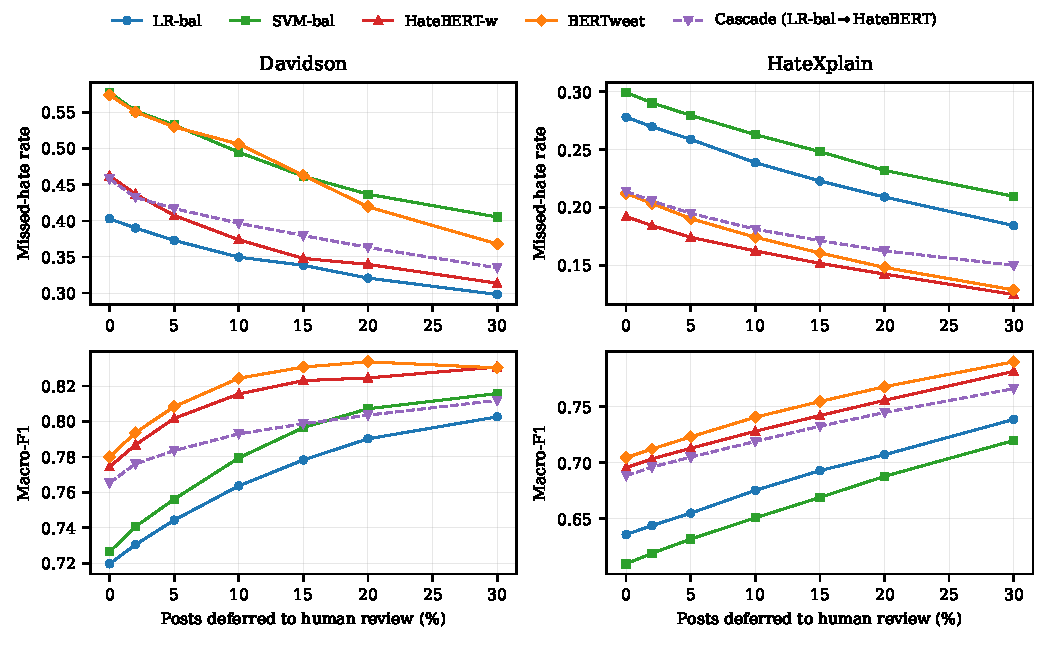
\includegraphics[width=0.92\textwidth]{figures/triage.pdf}
\caption{Missed-hate rate (top) and macro-F1 (bottom) as the share of posts deferred to a simulated human moderator grows from 0 to 30\% (mean over five splits and 20 moderator draws). The cascade applies LR-bal first and escalates its low-confidence posts to HateBERT.}
\label{fig:triage}
\end{figure*}

\begin{table*}[t]
\centering
\caption{Human--AI Systems at a 10\% Review Budget (Mean Over Splits). Human = One Randomly Drawn Real Annotator Vote per Deferred Post; Oracle = Gold Label. MHR = Missed-Hate Rate; FFR = False Hate-Flag Rate Among Non-Hate Posts; Cost = Expected Cost per Post With $c_m=5$; GPU = Share of Posts Processed by a Transformer.}
\label{tab:triage}
\small
\setlength{\tabcolsep}{3.5pt}
\begin{tabular}{l|ccccc|ccccc}
\toprule
 & \multicolumn{5}{c|}{Davidson} & \multicolumn{5}{c}{HateXplain} \\
System & Macro-F1 & MHR & FFR & Cost & GPU\,\% & Macro-F1 & MHR & FFR & Cost & GPU\,\% \\
\midrule
LR-bal & 0.720 & 0.403 & 0.085 & 0.218 & 0 & 0.636 & 0.278 & 0.122 & 0.607 & 0 \\
LR-bal + human & 0.764 & 0.350 & 0.065 & 0.199 & 0 & 0.675 & 0.239 & 0.106 & 0.547 & 0 \\
SVM-bal + human & 0.779 & 0.495 & 0.033 & 0.208 & 0 & 0.651 & 0.263 & 0.119 & 0.596 & 0 \\
HateBERT-w & 0.774 & 0.462 & 0.040 & 0.187 & 100 & 0.696 & 0.192 & 0.114 & 0.456 & 100 \\
HateBERT-w + human & 0.816 & 0.374 & 0.033 & 0.171 & 100 & 0.728 & 0.162 & 0.105 & 0.414 & 100 \\
BERTweet & 0.780 & 0.574 & 0.022 & 0.199 & 100 & 0.705 & 0.212 & 0.100 & 0.472 & 100 \\
BERTweet + human & 0.824 & 0.506 & 0.013 & 0.188 & 100 & 0.741 & 0.174 & 0.090 & 0.418 & 100 \\
Cascade + human & 0.793 & 0.397 & 0.041 & 0.187 & 19 & 0.719 & 0.181 & 0.101 & 0.443 & 42 \\
HateBERT-w + oracle & 0.864 & 0.287 & 0.022 & 0.133 & 100 & 0.748 & 0.145 & 0.097 & 0.377 & 100 \\
BERTweet + oracle & 0.897 & 0.367 & 0.002 & 0.135 & 100 & 0.762 & 0.155 & 0.081 & 0.378 & 100 \\
\bottomrule
\end{tabular}

\end{table*}

\textbf{Review closes the accuracy gap.} Fig.~\ref{fig:triage} and Table~\ref{tab:triage} show that deferring uncertain posts steadily raises macro-F1. With 10\% review, LR-bal rises from 0.720 to 0.764 and BERTweet from 0.780 to 0.824 on Davidson. A CPU-only SVM-bal with 10\% review reaches 0.779, matching BERTweet working alone (0.780). On HateXplain, LR-bal needs about 20\% review to match BERTweet alone (0.707 vs.\ 0.705). For platforms without GPU infrastructure, human review time can therefore substitute for model capacity, at a quantifiable rate.

\textbf{Review does little for missed hate.} Missed hate falls much more slowly. Reviewing 10\% of posts lowers the MHR of LR-bal from 0.403 to 0.350 and of BERTweet from 0.574 to 0.506 on Davidson. Even an error-free reviewer of the same 10\% leaves BERTweet missing 36.7\% of hate. Most missed hate is labeled offensive with high confidence, so it never enters the review queue. Confidence-based deferral improves overall accuracy, but it is not aimed at the errors that matter most.

\textbf{The human is imperfect.} A single annotator agrees with the majority label at macro-F1 0.802 (Davidson) and 0.831 (HateXplain). The gap between annotator and oracle review is correspondingly large on Davidson (BERTweet + human 0.824 vs.\ + oracle 0.897), so evaluations that assume a perfect moderator overstate what deferral achieves.

\textbf{Cascades save GPU work.} Applying LR-bal first and escalating only its low-confidence posts to HateBERT (threshold chosen on validation, 0.66--0.76 on Davidson and 0.54--0.62 on HateXplain) sends 19\% and 42\% of posts to the GPU. Without review, this costs 0.007 and 0.008 macro-F1 relative to HateBERT on every post (0.765 vs.\ 0.772; 0.688 vs.\ 0.696). With 10\% review, the cascade also has a lower MHR than BERTweet on Davidson (0.397 vs.\ 0.506), because LR-bal's higher hate recall carries through.

\begin{table}[t]
\centering
\caption{Cost-Minimizing Review Budget $b^{*}$ and Expected Cost per Post $J(b^{*})$ as the Cost of Missed Hate $c_m$ Grows (Mean Over Splits; Budgets Searched Up to 30\%). Bold: Lowest Cost.}
\label{tab:cost}
\scriptsize
\setlength{\tabcolsep}{4pt}
\begin{tabular}{ccccc}
\toprule
$c_m$ & LR-bal & HateBERT-w & BERTweet & Qwen2.5-3B \\
\midrule
\multicolumn{5}{l}{\textit{Davidson}} \\
1 & 11\% / 0.118 & 3\% / 0.079 & \textbf{2\% / 0.065} & 30\% / 0.356 \\
2 & 12\% / 0.138 & 4\% / 0.103 & \textbf{3\% / 0.097} & 30\% / 0.364 \\
5 & 16\% / 0.197 & \textbf{12\% / 0.170} & 10\% / 0.185 & 30\% / 0.386 \\
10 & 23\% / 0.288 & \textbf{14\% / 0.270} & 26\% / 0.308 & 30\% / 0.424 \\
20 & 27\% / 0.463 & \textbf{25\% / 0.462} & 30\% / 0.521 & 30\% / 0.498 \\
\midrule
\multicolumn{5}{l}{\textit{HateXplain}} \\
1 & 24\% / 0.247 & 16\% / 0.213 & \textbf{17\% / 0.202} & 30\% / 0.419 \\
2 & 30\% / 0.304 & 25\% / 0.254 & \textbf{23\% / 0.246} & 30\% / 0.443 \\
5 & 30\% / 0.474 & 30\% / 0.371 & \textbf{30\% / 0.367} & 30\% / 0.514 \\
10 & 30\% / 0.759 & \textbf{30\% / 0.563} & 30\% / 0.566 & 30\% / 0.633 \\
20 & 30\% / 1.328 & 30\% / 0.949 & 30\% / 0.963 & \textbf{30\% / 0.871} \\
\bottomrule
\end{tabular}

\end{table}

\textbf{Cost.} Table~\ref{tab:cost} turns these trade-offs into a decision. When missed hate costs no more than twice a false flag, BERTweet with almost no review (2--3\%) is cheapest on Davidson. Once missed hate costs five times a false flag or more, class-weighted HateBERT becomes cheapest, and at $c_m=20$ the CPU-only LR-bal (0.463) matches it (0.462) while BERTweet costs 13\% more (0.521). The optimal review budget grows with $c_m$, from 2--11\% to 25--30\%. On HateXplain, where hate is common and the transformers' hate recall is high, the transformers are cheapest for $c_m\le10$ and LR-bal costs 22--40\% more. Only when missed hate costs twenty times a false flag does the over-flagging LLM become cheapest (0.871 vs.\ 0.949 for HateBERT-w); on Davidson it is never competitive. The optimal budget on HateXplain reaches the largest value we searched (30\%) for $c_m\ge5$, so the true optimum may be higher.

\subsection{RQ3: Who Bears the Errors?}\label{sec:rq3}
\begin{table}[t]
\centering
\caption{Dialect Disparity on Davidson (Posterior Threshold 0.5; Mean Over Splits). FHF = False Hate-Flag Rate Among Non-Hate Tweets; FAF = False Abusive-Flag Rate (Hate or Offensive) Among Tweets Labeled Neither; Deferred = Share of the Group's Tweets Sent to Review. AAE/WAE = Ratio of Group Means.}
\label{tab:dialect}
\scriptsize
\setlength{\tabcolsep}{3.5pt}
\begin{tabular}{llcccc}
\toprule
 & & \multicolumn{2}{c}{No review} & \multicolumn{2}{c}{10\% review} \\
Model & Group & FHF & FAF & FAF & Deferred \\
\midrule
\multirow{3}{*}{LR-bal} & AAE & 0.069 & 0.222 & 0.177 & 0.081 \\
 & WAE & 0.098 & 0.047 & 0.031 & 0.142 \\
 & AAE/WAE & \textbf{0.70} & \textbf{4.73} & \textbf{5.72} & \textbf{0.57} \\ \midrule
\multirow{3}{*}{Linear SVM-bal} & AAE & 0.024 & 0.315 & 0.230 & 0.057 \\
 & WAE & 0.062 & 0.076 & 0.046 & 0.182 \\
 & AAE/WAE & \textbf{0.38} & \textbf{4.17} & \textbf{4.97} & \textbf{0.31} \\ \midrule
\multirow{3}{*}{HateBERT-w} & AAE & 0.015 & 0.246 & 0.179 & 0.081 \\
 & WAE & 0.057 & 0.048 & 0.027 & 0.136 \\
 & AAE/WAE & \textbf{0.26} & \textbf{5.13} & \textbf{6.54} & \textbf{0.60} \\ \midrule
\multirow{3}{*}{BERTweet} & AAE & 0.007 & 0.326 & 0.273 & 0.048 \\
 & WAE & 0.037 & 0.056 & 0.033 & 0.157 \\
 & AAE/WAE & \textbf{0.19} & \textbf{5.81} & \textbf{8.23} & \textbf{0.31} \\ \bottomrule
\end{tabular}

\end{table}

\begin{table}[t]
\centering
\caption{Robustness of the Dialect Result: AAE/WAE Ratio of False Abusive-Flag Rates Without $\to$ With 10\% Review, at Three Posterior Thresholds}
\label{tab:robust}
\scriptsize
\setlength{\tabcolsep}{4pt}
\begin{tabular}{lccc}
\toprule
Posterior threshold & 0.5 & 0.6 & 0.7 \\
\midrule
LR-bal & 4.73$\to$5.72 & 7.01$\to$8.54 & 7.90$\to$11.40 \\
Linear SVM-bal & 4.17$\to$4.97 & 6.29$\to$6.38 & 5.75$\to$7.20 \\
HateBERT-w & 5.13$\to$6.54 & 8.08$\to$10.60 & 9.15$\to$10.88 \\
BERTweet & 5.81$\to$8.23 & 7.21$\to$11.30 & 7.79$\to$12.15 \\
\midrule
AAE / WAE per split & 1633 / 727 & 1021 / 336 & 499 / 105 \\
\bottomrule
\end{tabular}

\end{table}

\textbf{Dialect.} Table~\ref{tab:dialect} shows that the dialect disparity lies in the offensive label rather than the hate label. Among tweets annotated as neither hateful nor offensive, all four systems flag AAE tweets as abusive at 4.2--5.8 times the rate of WAE tweets. False \emph{hate} flags, by contrast, are lower for AAE (ratios 0.19--0.70), as is the gold hate rate (3.8\% vs.\ 7.8\%).

\textbf{Review widens the gap.} Confidence-based deferral sends WAE tweets to review 1.7--3.3 times as often as AAE tweets: the models are confident, and frequently wrong, about AAE. Review lowers the false abusive-flag rate of AAE tweets in absolute terms (e.g., 0.326 to 0.273 for BERTweet), but it lowers that of WAE tweets proportionally more (0.056 to 0.033). As a result, the AAE/WAE ratio rises for all four systems, from 5.81 to 8.23 for BERTweet and from 4.73 to 5.86 for LR-bal. Table~\ref{tab:robust} shows that the widening holds at stricter dialect thresholds, where the disparity itself is larger, in 11 of 12 model--threshold combinations (the exception is SVM-bal at threshold 0.6, 6.29 to 6.00). A deferral policy that looks neutral thus directs human attention away from the community the model is already biased against. Because the gold labels and the simulated moderators come from the same annotators whose judgments show this bias \cite{sap2019risk}, these measured error rates likely understate the true disparity.

\begin{table}[t]
\centering
\caption{Missed-Hate Rate by Targeted Community on HateXplain With 0\% and 10\% Review (Mean Over Splits). Hate Posts: Mean Number per Test Split. $^{*}$Fewer Than 50 Hate Posts per Split; Interpret With Caution.}
\label{tab:targets}
\scriptsize
\setlength{\tabcolsep}{3pt}
\begin{tabular}{lccccccc}
\toprule
 & Hate & \multicolumn{2}{c}{LR-bal} & \multicolumn{2}{c}{HateBERT-w} & \multicolumn{2}{c}{BERTweet} \\
Target & posts & 0\% & 10\% & 0\% & 10\% & 0\% & 10\% \\
\midrule
African & 451 & 0.177 & 0.152 & 0.102 & 0.088 & 0.113 & 0.097 \\
Jewish & 267 & 0.149 & 0.122 & 0.119 & 0.099 & 0.129 & 0.096 \\
Islam & 248 & 0.309 & 0.262 & 0.187 & 0.148 & 0.212 & 0.163 \\
Homosexual & 145 & 0.429 & 0.381 & 0.372 & 0.334 & 0.387 & 0.342 \\
Arab & 102 & 0.190 & 0.166 & 0.111 & 0.080 & 0.110 & 0.075 \\
Women & 82 & 0.439 & 0.357 & 0.317 & 0.297 & 0.313 & 0.280 \\
Hispanic$^{*}$ & 47 & 0.217 & 0.192 & 0.075 & 0.079 & 0.064 & 0.056 \\
Refugee$^{*}$ & 38 & 0.625 & 0.548 & 0.486 & 0.334 & 0.446 & 0.334 \\
Asian$^{*}$ & 34 & 0.395 & 0.306 & 0.233 & 0.196 & 0.374 & 0.267 \\
\bottomrule
\end{tabular}

\end{table}

\textbf{Targeted communities.} Table~\ref{tab:targets} shows that how much hate is missed depends strongly on whom it targets. Among the six groups with at least 80 hate posts per split, HateBERT-w misses 10--12\% of hate against African, Arab, and Jewish people but 32\% against women and 37\% against homosexual people, and LR-bal misses more in every group. Ten percent review lowers the rate for each of these six groups but leaves the broad ordering unchanged. Rates for refugees, Asian people, and Hispanic people rest on fewer than 50 posts per split and are reported only for completeness.

\subsection{Compute}
\begin{table}[t]
\centering
\caption{Compute per Split (Davidson / HateXplain): Training Time, Inference Time, and Measured Peak GPU Memory. $^{a}$From the Scoring Log (About 620\,s per 1{,}000 Posts). $^{b}$Size of the 16-Bit Model Weights, Not a Measured Peak.}
\label{tab:compute}
\scriptsize
\setlength{\tabcolsep}{2.4pt}
\begin{tabular}{llccc}
\toprule
Model & Hardware & Training & Inference & Peak GPU \\
 & & (per split) & (ms/post) & memory (GB) \\
\midrule
LR-bal & CPU & 1.4\,s / 2.5\,s & $<$0.01 & -- \\
Linear SVM-bal & CPU & 0.2\,s / 0.2\,s & $<$0.01 & -- \\
GA search (LR/MNB) & CPU & 4.3\,min / 3.8\,min & $<$0.01 & -- \\
BPSO + LR-bal & CPU & 3.1\,min / 2.8\,min & $<$0.01 & -- \\
RoBERTa & T4 GPU & 4.8\,min / 4.6\,min & 0.70 / 1.03 & 2.4 / 2.4 \\
BERTweet & T4 GPU & 5.0\,min / 4.9\,min & 0.83 / 1.22 & 2.1 / 2.5 \\
HateBERT & T4 GPU & 4.1\,min / 3.7\,min & 0.71 / 1.07 & 1.9 / 2.2 \\
HateBERT-w & T4 GPU & 4.2\,min / 3.8\,min & 0.71 / 1.07 & 1.9 / 2.2 \\
Qwen2.5-3B (zero-shot) & T4 GPU & -- & 531 / $\approx$620$^{a}$ & 6.2$^{b}$ \\
\bottomrule
\end{tabular}

\end{table}

Table~\ref{tab:compute} lists measured compute. Class-weighted linear models train in seconds on CPU. Each transformer fine-tunes in about 4--5 minutes on a T4 and uses at most 2.6\,GB of GPU memory, with inference of 0.7--1.2\,ms per post. The genetic and swarm searches each take 3--4 CPU-minutes per split without improving on the default class-weighted model. The zero-shot LLM needs no training but is roughly 500--750 times slower than the fine-tuned transformers at inference (about 0.5--0.6\,s per post), so scoring one corpus took several GPU-hours.

% =====================================================================
\section{Discussion}
% =====================================================================
\textbf{Evaluate moderation systems on missed hate.} Macro-F1 ranks unweighted transformers first on Davidson, yet those models miss more hate than a class-weighted logistic regression. A platform choosing a model by macro-F1 alone could deploy the system that leaves the most hate online. Class weighting is the single most consequential modeling choice we observed, for linear models and transformers alike, and it costs nothing.

\textbf{Human review buys accuracy, not hate recall.} Review time can substitute for model capacity: 10--20\% review brings CPU models to the accuracy of a transformer working alone, which matters for small platforms and moderation teams without GPU infrastructure. But deferring the least-confident posts mostly corrects errors between offensive and neither, while confidently missed hate stays unreviewed. Deferral policies that target the hate class directly, for example by deferring posts whose hate probability lies in an uncertain band, or learned deferral policies \cite{madras2018predict,mozannar2020consistent}, are a natural next step.

\textbf{Audit who receives human attention.} Because confidence is lower for WAE tweets, a confidence-based queue gives WAE speakers more access to human judgment and AAE speakers more automated decisions. The disparity in false abusive flags then grows with the review budget. Platforms should audit deferral rates by group, not only error rates, and could consider group-stratified review quotas.

\textbf{Pipeline complexity and leakage.} Swarm feature selection, genetic tuning, and sentiment-driven fuzzy post-processing add computation without improving on a class-weighted linear model, and a test-set leak of the size we measured would be enough to make some of them appear useful.

\subsection{Ethical Considerations}
This study uses only publicly released, de-identified research datasets and collects no new data. Example posts are not reproduced. Dialect labels are statistical estimates of language variety used only in aggregate; they are not inferences about any individual's race. Human moderators are simulated from existing crowd annotations, so no person was exposed to additional harmful content. Better automated detection can also be used for over-broad removal of speech; our cost framework makes the trade-off between missed hate and false flags explicit rather than hiding it in a single metric.

\subsection{Limitations}
The simulated moderator is a crowd annotator rather than a trained moderator applying platform policy, and because the majority label includes that annotator's vote, agreement with the gold label is optimistic. Gold labels themselves carry annotator bias, especially for AAE \cite{sap2019risk}, so error rates measured against them are an imperfect proxy for harm. Cost values are illustrative policy parameters, which is why we sweep them, and on HateXplain the cost-minimizing budget reached the largest value we searched. Both corpora are English and predate current platform language. Dialect groups depend on a posterior threshold, which we vary, and three target groups have too few hate posts for firm conclusions. Swarm search used the original pipeline's configuration; other initializations or transfer functions might let it change the subset size. The LLM baseline uses a single 3B-parameter model and a single zero-shot prompt; larger models, few-shot prompting, or fine-tuning would likely perform better. Finally, deferral uses the simplest confidence rule.

% =====================================================================
\section{Conclusion}
% =====================================================================
Evaluated as part of a moderation pipeline rather than in isolation, hate speech classifiers look different. Fine-tuned transformers are clearly more accurate than classical models, and a small zero-shot LLM is no substitute for either, but class weighting decides how much hate is caught, and macro-F1 alone can pick the system that misses most. Human review of uncertain posts lets inexpensive models match transformer accuracy, yet it barely touches confidently missed hate and, by directing attention toward WAE tweets, widens the dialect disparity in false abusive flags. The swarm, genetic, and fuzzy components of a published multi-stage pipeline add nothing over class weighting, and test-set fitness inflates results by about 0.01. Future work should study deferral policies aimed at the hate class and at equitable allocation of review, real moderators rather than simulated ones, and multilingual platforms.

\section*{Data and Code Availability}
All code, including the scripts that generate every table in this paper from the experiment outputs, is available at \url{https://github.com/jeevan-aizen/research_paper_tcss}. The datasets are available from their original authors \cite{davidson2017automated,mathew2021hatexplain}.

\section*{Acknowledgment}
The authors thank the Department of Computer Science and Engineering (AI\&ML), Geethanjali College of Engineering and Technology, Hyderabad, for institutional support. \res{AI-use disclosure required by IEEE, e.g.: ``Claude (Anthropic) was used to assist with drafting and editing portions of this manuscript and the experiment code; all experiments were run, and all results verified, by the authors.'' Edit to reflect actual use.}

\bibliographystyle{IEEEtran}
\bibliography{refs}

\begin{IEEEbiography}[{\includegraphics[width=1in,height=1.25in,clip,keepaspectratio]{jeevan.png}}]{Kolla Jeevan}
received the B.Tech.\ degree in computer science and engineering (AI\&ML) from Geethanjali College of Engineering and Technology, Hyderabad, India, in 2024. He is currently working as an AI Engineer. His research interests include natural language processing, large language model-based agentic systems, hate speech detection, and MLOps. He has an IEEE Access publication on genetic algorithms for fraud detection and a filed patent on image enhancement for OCR. ORCID: \res{Jeevan's ORCID}.
\end{IEEEbiography}

\begin{IEEEbiography}[{\includegraphics[width=1in,height=1.25in,clip,keepaspectratio]{abhinay.png}}]{V. S. Abhinay Paul}
received the B.Tech.\ degree in computer science and engineering from Geethanjali College of Engineering and Technology, Hyderabad, India, in 2024. His research interests include natural language processing, transformer models, and bio-inspired optimization techniques applied to text classification. ORCID: 0009-0004-6726-2272.
\end{IEEEbiography}

\begin{IEEEbiography}[{\includegraphics[width=1in,height=1.25in,clip,keepaspectratio]{professor.png}}]{Angotu Nageswara Rao}
(Member, IEEE) received the Ph.D.\ degree in computer science and engineering. He is currently an Associate Professor and Head of the Department of Computer Science and Engineering (AI\&ML), Geethanjali College of Engineering and Technology, Hyderabad, India. His research interests include artificial intelligence, machine learning, natural language processing, and cybersecurity. He has published several papers in reputed international journals and conferences. ORCID: 0000-0002-8413-5994.
\end{IEEEbiography}

\end{document}
